\textbf{Метод 3 --- МНК--аппроксимация}\\

\textbf{Задание}

Для таблично заданной функции путем решения нормальной системы МНК найти приближающие многочлены а) 1--ой и б) 2--ой степени. Для каждого из приближающих многочленов вычислить вычислить сумму квадратов ошибок. Построить графики приближаемой функции и приближающих многочленов.\\

\textbf{Вариант:} 3

\begin{tabular}{|c|c|c|c|c|c|c|}
\hline
i & 0 & 1 & 2 & 3 & 4 & 5\\
\hline
$x_i$ & -0.9 & 0.0 & 0.9 & 1.8 & 2.7 & 3.6 \\
\hline
$y_i$ & -0.36892 & 0.0 & 0.36892 & 0.85408 & 1.7856 & 6.3138 \\
\hline
\end{tabular}
\vspace{0.5cm}

\textbf{Описание алгоритма}

Пусть задана таблично в узлах $x_j$ функция $y_j=f(x_j), j=0,1,...,N$. При этом значения функции $y_j$ определены с некоторой погрешностью, также из физических соображений известен вид функции, которой должны приближенно удовлетворять табличные точки, например: многочлен степени $n$, у которого неизвестны коэффициенты $a_i, F_n(x)=\sum\limits_{i=0}^na_ix^i$. Неизвестные коэффициенты будем находить из условия минимума квадратичного отклонения многочлена от таблично заданной функции.

$$
\Phi=\sum\limits_{j=0}^N[F_n(x_j)-y_j]^2
$$

Минимума $\Phi$ можно добиться только за счет изменения коэффициентов многочлена $F_n(x)$. Необходимые условия экстремума имеют вид\\

$$
\frac{\partial \Phi}{\partial a_k}=2\sum\limits_{j=0}^N[\sum\limits_{i=0}^na_ix_j^i-y_j]x_j^k=0, k=0,1,...,n
$$

Эту систему для удобства преобразуют к следующему виду:

$$
\sum\limits_{i=0}^na_i\sum\limits_{j=0}^Nx_j^{k+i}=\sum\limits_{j=0}^Ny_jx_j^k, k=0,1,...,n
$$

Затем нужно решить систему и, тем самым, получить коэффициенты $a_0, a_1, ..., a_n$ для полинома.\\

\textbf{Реализация}
\begin{lstlisting}
#include "./dependens/TSolve.h"
#include <fstream>
#include <functional>

using namespace std;

static size_t powMNK = 2;

int ToInt(const string& str) {
	int res = 0;
	for (int i = str.length() - 1; i >= 0 ; --i) {
		res = res * 10 + (str[i] - '0');
	}
	return res;
}

int main(int argc, char* argv[]) {
	if (argc != 3) {
		cerr << "Error: arg is incorrect" << endl;
		exit(-1);
	}
	string dataFile = argv[1];
	powMNK = max(0, ToInt(argv[2]));
	ifstream in(dataFile, ios::in);

	size_t N;
	vector<double> X, Y;
	double temp;
	
	in >> N;
	for (size_t i = 0; i < N; ++i) {
		in >> temp;
		X.push_back(temp);
	}
	for (size_t i = 0; i < N; ++i) {
		in >> temp;
		Y.push_back(temp);
	}
	in.close();

	TMatrix matrixFI(N, powMNK + 1, Zero);
	for (size_t i = 0; i < N; ++i) {
		for (size_t j = 0; j < powMNK + 1; ++j) {
			matrixFI[i][j] = pow(X[i], 1.0 * j);
		}
	}
	TVector vecY(Y);
	string inputData 	= "./dependens/inputData";
	string outputData 	= "./dependens/outputData";
	ofstream input(inputData, ios::out);
	ifstream output(outputData, ios::in);
	TSolve solution(inputData, outputData);
 
	TMatrix writeMatrix = matrixFI.Rotate() * matrixFI;
	TVector writeVector = (matrixFI.Rotate() * vecY.Rotate()).Rotate();
	input << powMNK + 1 << endl;
	for (size_t j = 0; j < writeMatrix.GetSizeRow(); ++j) {
		for (size_t i = 0; i < writeMatrix.GetSizeCol(); ++i) {
			input << writeMatrix[j][i] << " ";
		}
		input << writeVector[j] << endl;
	}
	if (!!solution.ToSolveByGauss()) {
		cerr << "Error: troubles with LUP method, check input data" << endl;
		exit(-1);
	}
	input.close();
	output.close();

	vector<double> aproxVec(powMNK + 1);
	in.open(outputData);

	for (size_t i = 0; i < aproxVec.size(); ++i) {
		in >> aproxVec[i];
	}
	in.close();

	auto CalcApproxFunction = [](double x, const vector<double>& arr) -> double {
		double res = 0.0;
		for (size_t i = 0; i < arr.size(); ++i)
			res += arr[i] * pow(x, 1.0 * i);
		return res;
	};

	string resultFile = "./solution3_3";
	ofstream o(resultFile, ios::out);

	o << "X: ";
	for (size_t i = 0; i < N; ++i) {
		o << X[i] << " ";
	}
	o << endl;
	o << "Y: ";
	for (size_t i = 0; i < N; ++i) {
		o << Y[i] << " ";
	}
	o << endl;
	o << "Approx koef: ";
	double sumOfError = .0;
	for (size_t i = 0; i < N; ++i) {
		o << CalcApproxFunction(X[i], aproxVec) << " ";
		sumOfError += (CalcApproxFunction(X[i], aproxVec) - Y[i]) * (CalcApproxFunction(X[i], aproxVec) - Y[i]);
	}	
	o << endl;
	o << "Summ of errors: " << sumOfError << endl;
	o.close();

	string pointFiles = "./plotDataPoint";
	string approxFiles = "./plotDataApprox" + to_string(powMNK);
	ofstream outPoint(pointFiles, ios::out);
	ofstream outApprox(approxFiles, ios::out);

	for (size_t i = 0; i < N; ++i) {
		outPoint << X[i] << " " << Y[i] << endl;
	}
	outPoint.close();
	double deltaX = 0.01;
	for (size_t i = 0; i < N - 1; ++i) {
		for (double cur = X[i]; cur <= X[i + 1]; cur += deltaX) {
			outApprox << cur << " " << CalcApproxFunction(cur, aproxVec) << endl;
		}
	}
	outApprox.close();
	return 0;
}
\end{lstlisting}
\vspace{0.5cm}

\textbf{Тестирование}\\

\textbf{Входной файл}
\begin{verbatim}
6
-0.9 0.0 0.9 1.8 2.7 3.6
-0.36892 0.0 0.36892 0.85408 1.7856 6.3138
\end{verbatim}

\textbf{Выходной файл}
\begin{verbatim}
-0.9 	-0.36892
0 		0
0.9 		0.36892
1.8 		0.85408
2.7 		1.7856
3.6 		6.3138
\end{verbatim}

\textbf{График}

\begin{center}
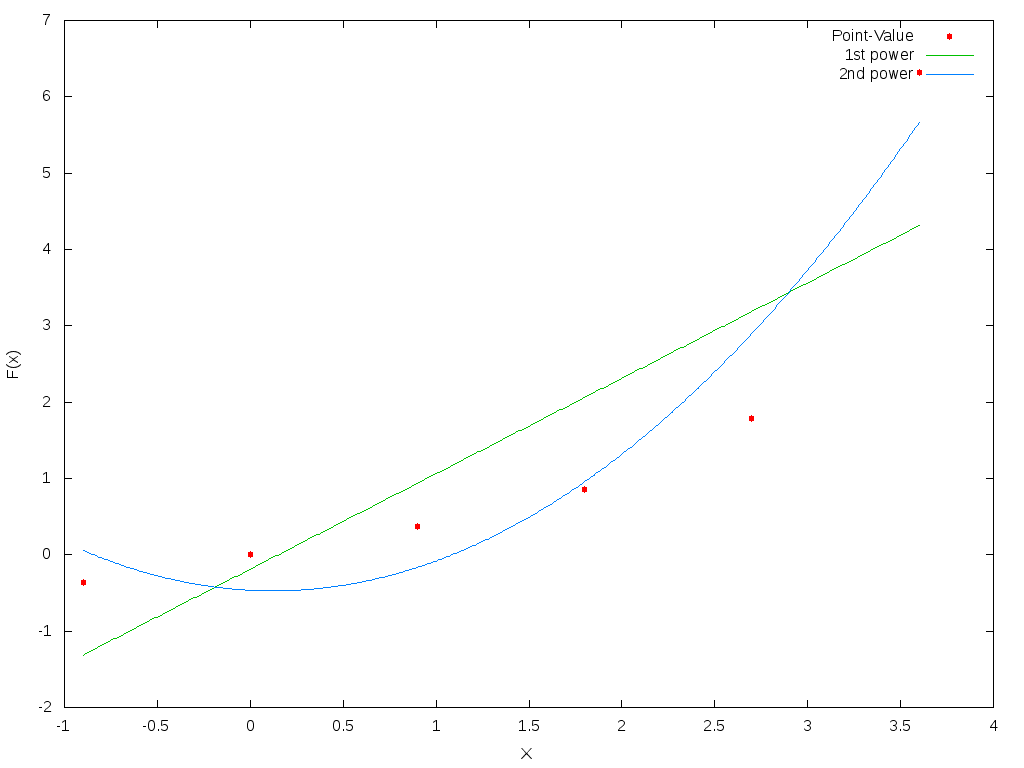
\includegraphics[scale=0.5]{images/graphic3_3.png}
\end{center}

\pagebreak
